\subsection{Headline result}
\label{subsec:headline-result}

Table~\ref{tab:phicpsi:prepost} collects the final validation angular MAE for every architecture, before and after the activation fix, against the analytic null.
The values are not merely \emph{close to} the null; they bracket it within a few hundredths of a radian in both directions, across seven architectures, two head parameterizations, and every $\lambda$.

One scope note belongs here rather than in the Discussion, because it bears on how to read every number below.
These are \emph{point} estimates under circular loss, and circular loss cannot distinguish ``no information'' from ``a genuinely multimodal or ridge-like true posterior that no single-valued output can express'' --- a sampler retains a meaningful joint posterior over $(\varphi_c, \psi)$ even where the degeneracy is exact (\S\ref{subsec:what-the-evidence-supports}).
The claim defended below is about point-estimation regression specifically, not about the information-theoretic content of the strain.

\begin{table}[tbp]
    \centering
    \caption{Validation angular MAE (rad) against the random-guessing
    null. ``Pre'' $=$ $\tanh$ outputs, Round~1; ``post'' $=$ linear
    outputs with $\lambda = 0.01$ where configured, Run~7 era. Dashes: no
    pre-fix run. Source: \texttt{pre\_post\_comparison.csv}.}
    \label{tab:phicpsi:prepost}
    \small
    \begin{tabular}{@{}lccccccc@{}}
        \toprule
        Head (null)             & TCN   & ResNet1D & CNN base & CNN attn & Inception & poc\_a & poc\_b \\
        \midrule
        $\varphi_c$ (1.571) pre & 1.572 & 1.564    & 1.577    & ---      & 1.556     & ---    & 1.572  \\
        $\varphi_c$ post        & 1.579 & 1.578    & 1.578    & 1.577    & 1.573     & 1.580  & 1.572  \\
        $\psi$ (0.785) pre      & 0.787 & 0.787    & 0.787    & ---      & 0.792     & 0.779  & 0.779  \\
        $\psi$ post             & 0.786 & 0.786    & 0.793    & 0.790    & 0.780     & 0.780  & 0.791  \\
        $\iota$ (1.571) post    & 1.544 & 1.588    & 1.570    & 1.559    & 1.571     & 1.560  & 1.573  \\
        \bottomrule
    \end{tabular}
\end{table}

The $\iota$ row is carried for diagnostic completeness, not as a positive control: as \S\ref{sec:phicpsi:pathology2} and \S\ref{sec:phicpsi:controls} establish, $\iota$ fails through a mechanism disjoint from the $\varphi_c/\psi$ pathologies, so its presence at the null here is neither confirming nor disconfirming evidence for the degeneracy claim.

What distinguishes models is not accuracy but \emph{failure style}, visible in the prediction distributions (Fig.~\ref{fig:phicpsi:hist}): poc\_a and tcn collapse most predictions onto one narrow mode ($r_{\mathrm{circ}} = 0.85$--0.86); poc\_b collapses almost totally ($r_{\mathrm{circ}} = 0.989$); cnn\_attention spreads its predictions broadly ($r_{\mathrm{circ}} = 0.43$ for $\varphi_c$, 0.17 for $\psi$) --- varied wrong answers instead of one constant wrong answer --- with ang\_MAE identical to everyone else's.
Output diversity is an architectural artifact; information recovery is uniformly nil.

\begin{figure}[tbp]
    \centering
    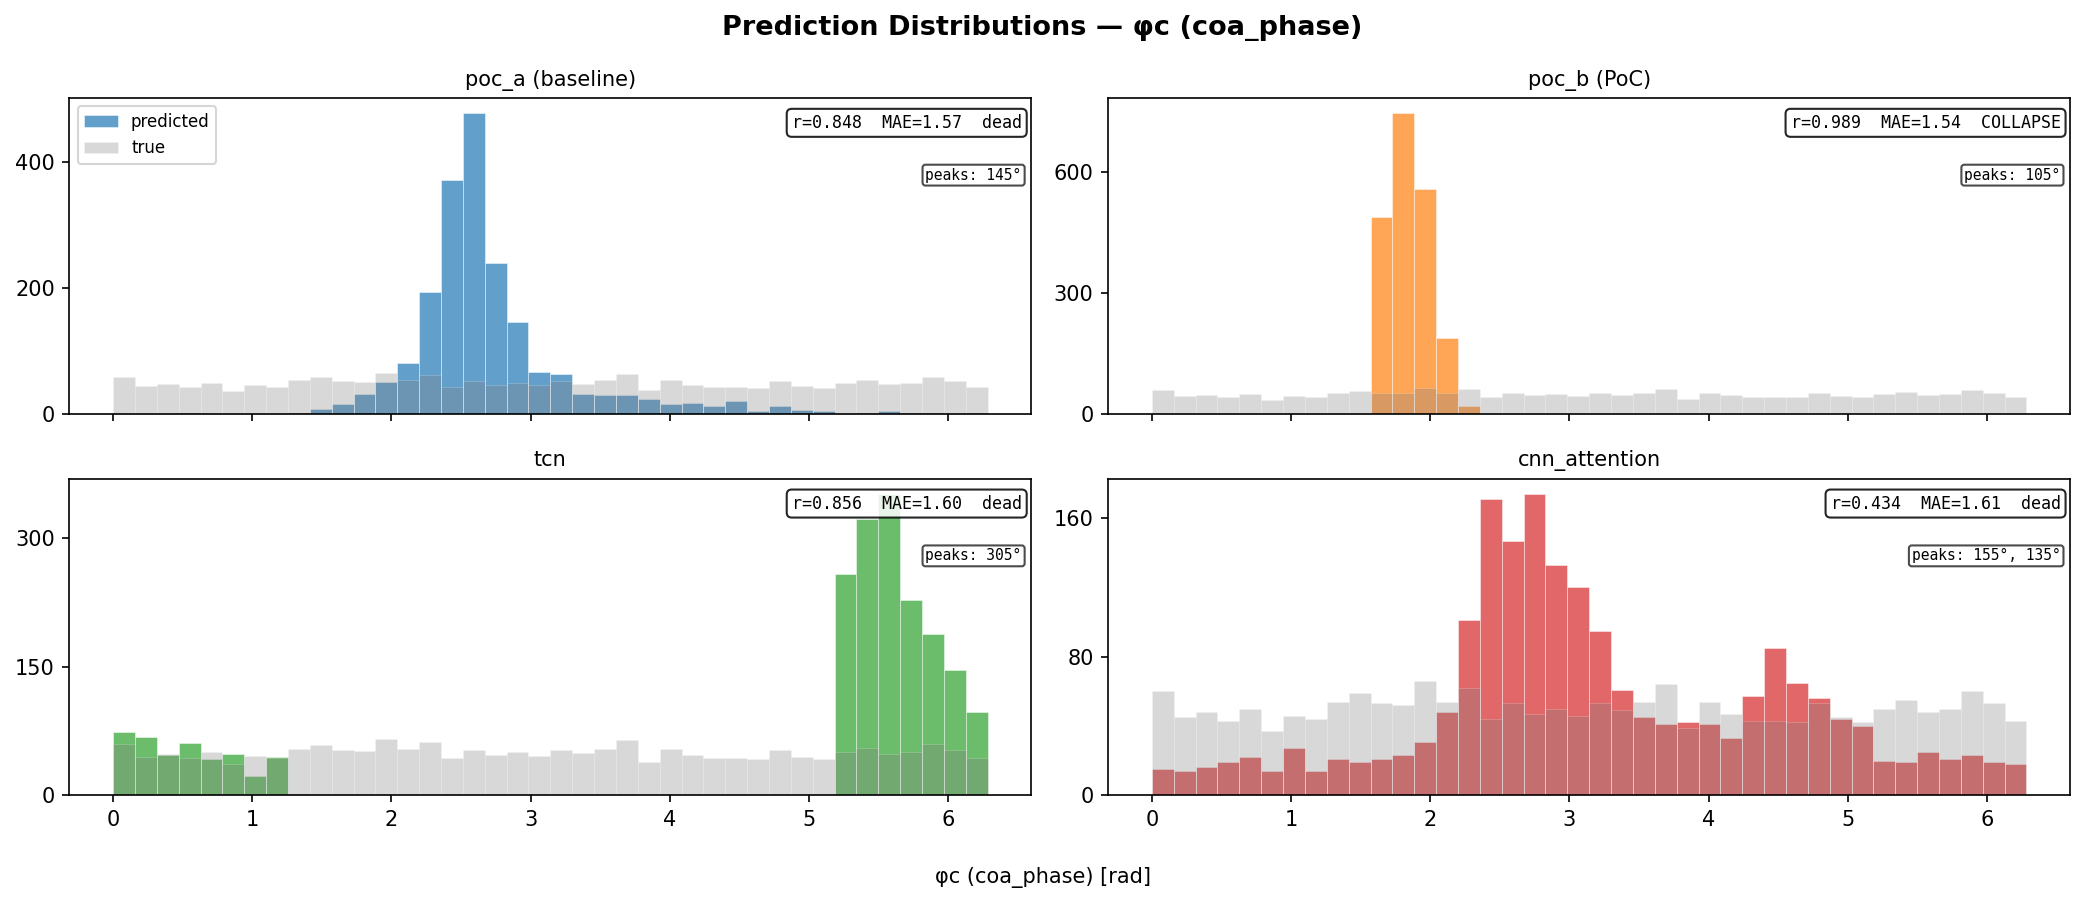
\includegraphics[width=\textwidth]{histogram_coa_phase_20260720_234304.png}
    \caption[Predicted $\varphi_c$ distributions]{Predicted $\varphi_c$ distributions (color) against the uniform truth (grey) for the four Run~7 models.
    Every model collapses to one or a few preferred angles ($r_{\mathrm{circ}} = 0.43$--0.99) while angular MAE sits at the null $\pi/2 \approx 1.571$ --- optimal constant-prediction behavior for an unidentifiable target.}
    \label{fig:phicpsi:hist}
\end{figure}

\subsection{Confound elimination}
\label{sec:phicpsi:confounds}

A five-section verification plan was executed against the Run~7 checkpoints under an explicit gating rule: nothing downstream counts as evidence about the degeneracy until the interpretability of the metrics themselves is established.
Table~\ref{tab:phicpsi:battery} summarizes.

\begin{table}[tbp]
    \centering
    \caption{Verification battery.}
    \label{tab:phicpsi:battery}
    \resizebox{\textwidth}{!}{
    \begin{tabular}{@{}llll@{}}
        \toprule
        \S  & Confound                            & Check                                 & Outcome                                                                                                                                                                                              \\
        \midrule
        A.1 & Penalty silently inactive           & config $+$ code-path inspection       & $\lambda = 0.01$ confirmed active in all four configs                                                                                                                                                \\
        A.2 & Magnitude drift invalidates metrics & full 80-epoch std\_ratio trajectories & 2/4 models fully healthy (poc\_b, cnn\_attention); tcn $\varphi_c$ still declining (0.34, $-0.0078$/epoch), poc\_a $\psi$ stable-but-low (0.44) $\to$ flagged, pursued in \S\ref{sec:phicpsi:prereg} \\
        A.3 & Gradient path dead                  & perturbation $+$ gradient-chain trace & path healthy; an $89\times$ prediction-sensitivity asymmetry initially flagged, provisionally closed by the calibrated standalone trace's paired-statistic channel (\S\ref{sec:phicpsi:asymmetry})                                                                    \\
        B   & poc\_b config bug                   & config diff vs poc\_a                 & four intentional keys only; worse collapse \emph{explained} by curriculum (below)                                                                                                                            \\
        C   & cnn\_attention hides real learning  & config diff $+$ architecture trace    & outlier metrics are attention-pooling variance artifacts; ang\_MAE at null                                                                                                                           \\
        D   & Sub-null MAE is real signal         & 10{,}000-permutation bootstrap        & 11/12 model$\times$head tests non-significant; $\varphi_c$ and $\psi$: 0/8                                                                                                                           \\
        E   & Learning hides in loud events       & SNR-tercile stratification            & no model--head pair shows a monotonic-and-material SNR trend                                                                                                                                         \\
        --- & Ordering-confounded bootstrap       & row-order audit                       & data i.i.d.\ (window variance ratio 0.991); artifact bound \SI{0.013}{\radian}                                                                                                                                \\
        \bottomrule
    \end{tabular}
    }
\end{table}

Two of these deserve narrative attention.

\paragraph{The poc\_b anomaly is consistent with the null but confounded by curriculum design.}
The combination-space model collapsed \emph{more} severely than its baseline twin ($r_{\mathrm{circ}}$ 0.989 vs 0.848).
The config diff shows only the four intended poc-mode keys; the mechanism is the curriculum itself.
For near-face-on samples $w(\iota) \approx 0$ suppresses the poorly-constrained combination, so the model effectively trains one combination --- a single constraint on the two-dimensional $(\varphi_c, \psi)$ --- and the optimal response to a single unlearnable constraint under circular loss is a sharp constant, which is what poc\_b produces (a single peak carrying ${\sim}42\%$ of all predictions).
The design would have exploited a breakable degeneracy; its collapse into the constant predictor is what that design does when the degeneracy is not breakable.
(Cost: a mild, predictable transfer-interference tax on chirp mass, MAE $0.977 \to 1.024$.)
The combination heads' own losses corroborate this at the loss level, not only the prediction-distribution level: combo A and combo B circular loss sat at $0.999 \to 0.999$ and $1.006 \to 0.991$ respectively through epoch 79 (\S\ref{sec:phicpsi:run7}) --- the random-guessing null --- so on the parameterization purpose-built to expose the analytically well-constrained combination, that combination's own loss never left the null either; the network did not merely fail to decouple $\varphi_c$ and $\psi$, it also failed to show measurable in-sample progress on the recoverable combination itself.
This reading is the best mechanistic account available, but it is not the only one: the curriculum's near-face-on suppression of one combination could itself produce rank-deficient gradients independent of whether the underlying target is truly unlearnable, so poc\_b is treated below (\S\ref{sec:phicpsi:pool}) as a distinct, curriculum-confounded consistency check rather than as an independent repeat of the certified null.

\paragraph{The cnn\_attention outlier is an artifact with a testable signature.}
Its lower $r_{\mathrm{circ}}$ comes from learned attention pooling producing higher-variance features than fixed GAP/GMP readouts --- spreading predictions without informing them (ang\_MAE 1.597, \emph{worst} of the four).
Its nominally significant inclination result is dissected below.

\subsection{Statistical significance}
\label{sec:phicpsi:bootstrap}

\begin{table}[tbp]
    \centering
    \caption{Label-permutation bootstrap ($N = 10{,}000$ shuffles,
        5{,}000 validation samples, one-sided). $z > 0$ means observed
        ang\_MAE beats the shuffled-null mean.
        Source: \texttt{bootstrap\_output/bootstrap\_ang\_mae\_20260721\_093533.md}.}
    \label{tab:phicpsi:bootstrap}
    \small
    \begin{tabular}{@{}lccc@{}}
        \toprule
        Model          & $\varphi_c$: $z$, $p$ & $\psi$: $z$, $p$ & $\iota$: $z$, $p$         \\
        \midrule
        poc\_a         & $-0.20$, 0.579        & $+0.46$, 0.324   & $+1.04$, 0.152            \\
        poc\_b         & $-1.25$, 0.895        & $-0.05$, 0.518   & $+0.07$, 0.464            \\
        tcn            & $-0.56$, 0.712        & $-0.33$, 0.630   & $+1.21$, 0.114            \\
        cnn\_attention & $-2.43$, 0.994        & $+0.07$, 0.472   & $\mathbf{+3.17,\ 0.0007}$ \\
        \bottomrule
    \end{tabular}
\end{table}

Eleven of twelve tests are non-significant (Table~\ref{tab:phicpsi:bootstrap}); \textbf{all eight $\varphi_c/\psi$ tests fail}, six of them on the \emph{worse-than-shuffled} side, and every one of the eight observed values falls inside its own null 95\% confidence interval (\texttt{bootstrap\_output/bootstrap\_ang\_mae\_20260721\_093533.md} reports the null CI directly for each; e.g.\ tcn/$\varphi_c$: observed 1.578 against null CI $[1.561, 1.588]$).
Across the eight $\varphi_c/\psi$ tests the null-CI half-widths range ${\approx}{}$\SIrange{0.002}{0.023}{\radian}, so this is not merely ``not significant'' --- it is a comparatively tight bound against even a small real effect for most model--head pairs.
The single nominal detection --- cnn\_attention on inclination --- is a genuine statistical outlier ($z=+3.17$, $p=0.0007$), and it \emph{does} survive Bonferroni correction across the twelve tests (threshold $p < 0.0042$; observed $p = 0.0007$ clears it) --- we do not dismiss it on multiple-comparisons grounds.
We do not treat it as counter-evidence to the degeneracy claim, because it fails the same test this paper applies to every other candidate signal: whether the effect grows with SNR.
Its effect size is $\Delta = {}$\SI{0.038}{\radian} (\ang{2.2}), and that effect is uniform across SNR terciles (1.526/1.548/1.527) --- flat, not increasing with signal strength.
This is not an ad hoc criterion invoked only here: it is the identical logic of the SNR stratification (\S\ref{sec:phicpsi:snr}) and of Step~3 of the pre-registered $\lambda$-retune gate (\S\ref{subsec:why-pre-register-an-engineering-sweep}), applied consistently --- a per-event phase-recovery effect must be stronger in louder events, while a population-level output-distribution bias need not be, and the inclination detection has the signature of the latter.
One honest scope limit: the SNR-monotonicity criterion was pre-registered as Step~3 of the \S\ref{subsec:why-pre-register-an-engineering-sweep} $\lambda$-retune gate specifically, not as a general-purpose rule for the bootstrap battery; applying the same logic here is principled --- it is the same physical argument, not a different one invented for this case --- but it was not itself locked in writing before this particular test, and the reader should weigh the dismissal accordingly rather than as a pre-registered result.
Read on its own terms rather than folded into the degeneracy verdict, this is a genuine anomaly --- possibly a population bias in this model's attention-pooling readout, possibly a real but weak effect specific to inclination --- and the honest report is that it does not generalize to either $\varphi_c$ or $\psi$, where all eight tests land at or worse than the shuffled null.
A row-ordering audit additionally bounded the largest possible ordering artifact at \SI{0.013}{\radian} and confirmed the permutation null is valid (validation data i.i.d.; window variance ratio 0.991).

\subsection{SNR stratification}
\label{sec:phicpsi:snr}

If weak phase information were present but diluted, it would concentrate in loud events.
It does not.
Across terciles (SNR $[7.0, 9.6]$ / $[9.7, 12.3]$ / $[12.3, 15.0]$, $n \approx 1{,}666$ each): every $\psi$ result lies within \SI{0.007}{\radian} of the null in every tercile for every model; three of four models are non-monotonic in $\varphi_c$; the single monotonic case (tcn: $1.633 \to 1.557 \to 1.543$) drops by \SI{0.090}{\radian} from low to high SNR --- larger than the \SI{0.038}{\radian} artifact scale established in \S\ref{sec:phicpsi:bootstrap}, and large enough that, read in isolation, it could look like a genuine SNR-dependent trend.
Two facts argue against that reading.
First, the more diagnostic comparison is not tercile-to-tercile but each tercile against the null (\SI{1.5708}{\radian}): the low tercile sits \emph{worse} than random guessing (1.633, $\Delta = -0.062$ vs null), and even the high tercile clears the null by only \SI{0.027}{\radian} --- itself beneath the artifact scale --- so the \SI{0.090}{\radian} swing is mostly the low tercile's anomalous departure \emph{from} the null, not the high tercile's departure \emph{toward} a genuine signal; a real degeneracy-breaking effect should make high-SNR predictions better than random, not merely less bad than an anomalously poor low-SNR estimate.
Second, tcn/$\varphi_c$ is the one model whose std\_ratio never converged to the healthy band (\S\ref{sec:phicpsi:prereg}) at $\lambda = 0.01$, so its ang\_MAE trend across any stratification is doubly uninterpretable as evidence of learning.

\subsection{Run 8: the $\lambda = 0$ ablation}
\label{sec:phicpsi:ablation}

One loose thread survived the battery: Run~7's validation circular losses \emph{rose} slightly over training ($+0.014$ to $+0.025$).
A rising loss could mean the magnitude penalty was actively corrupting predictions --- an engineering artifact worth fixing, not more null evidence --- so the two TCN-trunk baselines were re-run with $\lambda = 0$ (Fig.~\ref{fig:phicpsi:lam0}; Table~\ref{tab:phicpsi:lam0}).

\begin{table}[tbp]
    \centering
    \caption{Endpoint drift of validation circular loss.}
    \label{tab:phicpsi:lam0}
    \small
    \begin{tabular}{@{}llccl@{}}
        \toprule
        Model  & Head        & $\Delta$ at $\lambda{=}0$ & $\Delta$ at $\lambda{=}0.01$ & Reading                                      \\
        \midrule
        poc\_a & $\varphi_c$ & $+0.0010$                 & $+0.0249$                    & artifact of $\lambda$ (resolved)             \\
        poc\_a & $\psi$      & $+0.0002$                 & $+0.0163$                    & artifact of $\lambda$ (resolved)             \\
        tcn    & $\varphi_c$ & $+0.0011$                 & $+0.0204$                    & artifact of $\lambda$ (resolved)             \\
        tcn    & $\psi$      & $\mathbf{+0.0072}$        & $+0.0136$                    & persists at half size --- unexplained, small \\
        \bottomrule
    \end{tabular}
\end{table}

Three of four drift signals vanish with the penalty off: the creep was a penalty/uncertainty-weighting interaction, not anti-learning.
The fourth (tcn $\psi$) persists at $+0.0072$ on a loss of ${\sim}1.0$ and is recorded as unexplained-but-small rather than forced into the majority pattern.
The ablation also confirmed it was genuinely an off-state --- without the penalty, std\_ratio diverged to 73--83 --- and final MAEs at $\lambda = 0$ landed on the same nulls as every other run ($\varphi_c \approx 1.579$; $\psi \approx 0.780$--0.785).

\begin{figure}[tbp]
    \centering
    \includegraphics[width=\textwidth]{lam0_ablation_trajectories.png}
    \caption[$\lambda = 0$ ablation]{$\lambda = 0$ ablation for poc\_a and tcn: validation/training circular loss and validation std\_ratio for $\varphi_c$ (top) and $\psi$ (bottom); $\lambda = 0$ (solid) vs the $\lambda = 0.01$ references (dashed).
    Removing the penalty eliminates the upward validation-loss drift (e.g.\ $+0.0010$ vs $+0.0249$ for poc\_a $\varphi_c$) but lets $\lVert\mathbf{v}\rVert$ diverge (std\_ratio $> 140$ at peak).
    Circular loss remains at $\approx 1.0$ in every configuration.}
    \label{fig:phicpsi:lam0}
\end{figure}


\subsection{Closing the last open probe: the $89\times$ sensitivity asymmetry}
\label{sec:phicpsi:asymmetry}

Verification item A.3 left one mechanistic loose end: after a single optimizer step, the periodic heads' predictions moved with relative change ${\sim}1.6 \times 10^{-2}$, some $89\times$ more than the converged chirp-mass head's $1.8 \times 10^{-4}$ --- movement a one-step snapshot cannot classify as slow learning or noise.
The multistep trace built to resolve this was gated behind the pre-registered stability gate and therefore never ran during the retune; after the retune closed, it was decoupled into a standalone script and executed against the Run~7 checkpoints (25 consecutive gradient steps on a fixed 128-sample batch, with predictions tracked on a disjoint 512-sample probe).

\begin{table}[tbp]
    \centering
    \caption{Standalone multistep perturbation trace, at the converged checkpoints (``final'') and after a fresh initialization plus ${\sim}$1-epoch warmup (``early'').
        net/sum is the ratio of net displacement to summed per-step displacements (random-walk reference $1/\sqrt{25} = 0.20$).
        $\Delta$ is the paired per-sample probe change over the 25 steps with its paired-SE $t$ statistic --- circular loss for $\varphi_c/\psi$, transformed-target MSE for mchirp.
        Source: \texttt{perturbation\_trace\_output/}.}
    \label{tab:phicpsi:trace}
    \small
    \begin{tabular}{@{}llccc@{}}
        \toprule
        Stage & Model & $\varphi_c$: net/sum, $\Delta$ ($t$) & $\psi$: net/sum, $\Delta$ ($t$) & mchirp: net/sum, $\Delta$ ($t$) \\
        \midrule
        final & poc\_a         & 0.30, $-0.018$ ($-0.9$) & 0.63, $+0.043$ ($+0.8$) & 0.04, $+0.021$ ($+4.2$) \\
        final & poc\_b         & 0.39, $-0.013$ ($-1.0$) & 0.23, $+0.004$ ($+1.7$) & 0.04, $+0.040$ ($+9.0$) \\
        final & tcn            & 0.92, $-0.010$ ($-0.2$) & 0.36, $+0.050$ ($+1.6$) & 0.03, $+0.017$ ($+4.3$) \\
        final & cnn\_attention & 0.41, $-0.044$ ($-1.1$) & 0.34, $+0.023$ ($+0.7$) & 0.19, $+0.065$ ($+4.4$) \\
        early & poc\_a         & 0.16, $-0.017$ ($-1.6$) & 0.14, $+0.004$ ($+0.1$) & 0.09, $\mathbf{-0.158}$ ($\mathbf{-5.2}$) \\
        early & poc\_b         & 0.08, $-0.006$ ($-0.7$) & 0.09, $+0.001$ ($+0.1$) & 0.13, $\mathbf{-0.129}$ ($\mathbf{-3.4}$) \\
        early & tcn            & 0.24, $-0.002$ ($-0.0$) & 0.15, $+0.035$ ($+0.6$) & 0.10, $\mathbf{-0.113}$ ($\mathbf{-4.1}$) \\
        early & cnn\_attention & 0.42, $+0.001$ ($+0.0$) & 0.37, $-0.031$ ($-0.6$) & 0.29, $\mathbf{-0.646}$ ($\mathbf{-8.5}$) \\
        \bottomrule
    \end{tabular}
\end{table}

Two observations (Table~\ref{tab:phicpsi:trace}) stand on arithmetic alone.
First, the asymmetry is real and now explained: the periodic heads' raw outputs move coherently and far (net/sum up to 0.92 against the 0.20 random-walk reference), while the converged scalar control barely moves net (net/sum 0.03--0.16; its positive cosine similarity is attributable to Adam momentum, which correlates consecutive steps for every head).
Second, the coherent movement is dominantly \emph{radial}, not angular: the circular loss depends only on the predicted angle, and its change over 25 steps is bounded by $|\Delta| \le 0.050$ on a loss of ${\approx}1.0$ while the raw displacement is a large fraction of the output norm --- large coherent raw movement with near-zero angular consequence is precisely the $\lVert\mathbf{v}\rVert$-magnitude dynamics of \S\ref{sec:phicpsi:pathology2}, and the two most directional cases (tcn/$\varphi_c$, poc\_a/$\psi$) are exactly the two heads with the known std\_ratio pathologies.

The first run of the trace was reviewed before acceptance, and the review reshaped the instrument itself; the sequence is reported in order because each step gates the next.
The review raised two objections: the positive control had failed --- mchirp, the best-learned head in the investigation ($R^2 \approx 0.96$ throughout), read AMBIGUOUS at every converged checkpoint, so the classifier could not distinguish a demonstrably learned head from a dead one --- and the probe-loss deltas lacked the correct \emph{paired} statistic (the first run recorded only means, and a marginal-SE comparison is invalid for a before/after change on the same fixed samples).
Both were remediated: per-sample paired statistics were added to the instrument, and a calibration stage was defined with a pre-stated criterion --- rerun the trace near the start of training (fresh initialization plus ${\sim}$1-epoch warmup, since per-epoch checkpoints were never saved), where a genuinely learning mchirp \emph{must} read directional, with failure defined to retire the classifier.

\textbf{The calibration failed its criterion --- and in failing, validated the measurement that matters.}
Early-stage mchirp never read directional (net/sum 0.09--0.29) \emph{while its probe MSE was collapsing at $t = -3.4$ to $-8.5$}, the strongest learning signal in the entire table: the displacement-geometry classifier labels the fastest-learning head ``noise-like.''
The mechanism is instructive --- learning is not rigid drift; per-step prediction deltas decorrelate as different samples' errors are corrected --- and the verdict is mechanical: per the pre-stated tree, the geometry classifier is retired and no directional/ambiguous verdict from either run is used.
The same run, however, constitutes a \emph{passed} positive control for the instrument's other channel: the paired probe-loss statistic detects early mchirp learning decisively in all four models, and on that validated channel every periodic head is null at both stages (early $|t| \le 1.6$, final $|t| \le 1.72$, signs mixed across models and heads).
The early stage is the sharper result: a within-run, stage-matched, positive-controlled contrast in which the same instrument, over the same 25 steps, watches mchirp learn steeply while $\varphi_c$ and $\psi$ sit at the random baseline.
The paired statistic also extinguishes the one nominal escalation trigger from the first run --- tcn/$\varphi_c$, directional at net/sum 0.92 with an apparently decreasing probe loss, measures $-0.0097 \pm 0.0491$ ($t = -0.20$) --- and the radial explanation of the original $89\times$ asymmetry stands on arithmetic independent of the retired classifier: raw periodic outputs move by a large fraction of their norm while the angular loss moves by at most $|0.050|$, and the two largest raw movers are the two known std\_ratio-pathology heads.

Two secondary observations complete the account.
First, the final-stage mchirp deltas are significantly \emph{positive} --- probe MSE worsens by $+0.017$ to $+0.065$ ($t = +4.2$ to $+9.0$) --- which is not a probe artifact but the expected signature of resuming training on a single fixed batch: at convergence the full-data gradient is ${\approx}0$ while the batch gradient is not, so 25 repeated steps move the head along batch-specific directions at the expense of the held-out optimum.
Three pieces of in-hand evidence support this reading over a data-loading quirk: the probe pipeline is stage-independent yet yields strongly negative deltas early and positive ones late; the gradient batch is disjoint from the probe by construction, so the degradation is genuine out-of-batch generalization loss; and the effect appears only on the head with a real strain-to-target mapping --- a converged optimum to be dragged away from.
Read as an unplanned second control, it strengthens the final-stage null: the paired channel demonstrably has the power to detect a real, if artifactual, effect at the converged stage --- and $\varphi_c/\psi$ still show nothing against that backdrop.
Second, on sensitivity: the per-combo minimum detectable effect (${\approx}2\times$ the paired SE) spans ${\approx}0.005$--$0.10$ loss units across the twelve cases, so the individual $\varphi_c/\psi$ point estimates (up to $|0.050|$) are non-significant partly because the single-batch probe design yields wide standard errors --- the final-stage per-combo null is ``not rejected and bounded at the few-percent level,'' not ``excluded to arbitrary precision.''
This is adequate for A.3's mechanistic role: the degeneracy verdict itself is carried independently by the $N = 10{,}000$ label-permutation bootstrap (\S\ref{sec:phicpsi:bootstrap}) and the SNR stratification (\S\ref{sec:phicpsi:snr}), not by this trace.

\textbf{A.3 is provisionally closed, pending replication on a fresh holdout set}: the $89\times$ asymmetry was radial movement without angular learning.
The disposition honors the pre-stated decision tree in order --- the calibration criterion failed, so the classifier it governed is retired --- and the closure is then re-founded, transparently post hoc, on the surviving channel, which carries its own passed control from the same run; that residual caveat is recorded in the threats-to-validity list rather than hidden.

\subsection{Inclination stratification: does the degeneracy weaken edge-on?}
\label{sec:phicpsi:inclination}

The one population slice never separately reported in the original verification battery is inclination itself.
The analytic study of \S\ref{sec:phicpsi:prereq} predicts the $\varphi_c/\psi$ degeneracy is exact face-on and only partially breakable edge-on, so a recoverable signal, if present, should concentrate there.
\texttt{inclination\_stratification.py} was run against the four $\lambda$-matched Run~7 checkpoints, splitting the 5{,}000-sample validation set into the same face-on ($|\cos\iota| > 0.9$, $n=1{,}442$), mixed ($0.5 \le |\cos\iota| \le 0.9$, $n=1{,}918$), and edge-on ($|\cos\iota| < 0.5$, $n=1{,}640$) bands used throughout \S\ref{sec:phicpsi:prereq}.

\begin{table}[tbp]
    \centering
    \caption{Inclination-stratified ang\_MAE, edge-on band vs null (rad). Positive $\Delta$ = edge-on ang\_MAE \emph{better} than the random-guessing null (ang\_MAE $<$ null); negative $\Delta$ = \emph{worse} than null.
    Source: \texttt{inclination\_output/inclination\_stratification\_20260723\_130630.md}.}
    \label{tab:phicpsi:inclination}
    \small
    \begin{tabular}{@{}lccc@{}}
        \toprule
        Model & $\varphi_c$ edge-on $\Delta$ vs null & $\psi$ edge-on $\Delta$ vs null & Same-model $\iota$-band noise floor ($\max|\Delta|$) \\
        \midrule
        poc\_a         & $+0.0241$ & $-0.0227$ & 0.0569 \\
        poc\_b         & $+0.0096$ & $+0.0054$ & 0.0215 \\
        tcn            & $-0.0407$ & $-0.0083$ & 0.0225 \\
        cnn\_attention & $-0.0087$ & $-0.0189$ & 0.0944 \\
        \bottomrule
    \end{tabular}
\end{table}

No model shows a cross-consistent, edge-on-favoring recovery of either angle.
Of the eight $\varphi_c/\psi$ deviations, the largest in the \emph{hoped-for} direction is poc\_a/$\varphi_c$ ($+{}$\SI{0.0241}{\radian}, and the only one of the eight monotonic across all three bands: $1.6042 \to 1.5623 \to 1.5467$); the largest in the \emph{anti} direction is tcn/$\varphi_c$ ($-{}$\SI{0.0407}{\radian}).

Neither is evidence of recovered signal, for the same reason \S\ref{sec:phicpsi:snr} already established for the SNR axis, extended here with a model-matched calibration.
Because inclination is itself a labeled quantity, each model's already-diagnosed, uninformative $\iota$ head (\S\ref{sec:phicpsi:pathology2}) provides a same-model, same-binning noise floor for exactly this stratification: $\iota$ carries no information about $\varphi_c/\psi$ by construction, so its own band-to-band swings measure how much a completely uninformative head fluctuates from finite-band sampling alone at these $N$.
That floor is \SI{0.0569}{\radian} for poc\_a, \num{0.0215} for poc\_b, \num{0.0225} for tcn, and \num{0.0944} for cnn\_attention (the last consistent with its already-diagnosed high-variance attention-pooling readout, \S\ref{sec:phicpsi:confounds}) --- and every $\varphi_c/\psi$ deviation above falls at or below its own model's floor, with one exception.
tcn/$\varphi_c$'s $-{}$\SI{0.0407}{\radian} edge-on deviation exceeds tcn's own \SI{0.0225}{\radian} floor, but in the \emph{worse-than-null} direction and on the one head this paper already flags as never achieving certified metric health (std\_ratio never converged, \S\ref{sec:phicpsi:confounds}, \S\ref{sec:phicpsi:prereg}): an unstable head producing an oversized swing, in the direction a real signal could not produce, is consistent with its documented instability, not a new finding.

One honest limit on this argument, raised on review: the $\iota$-noise-floor comparison is a \emph{diagnostic calibration}, not a formal statistical test, and it assumes $\iota$'s band-to-band fluctuation is independent sampling noise rather than a symptom shared with $\varphi_c/\psi$'s own failure --- e.g.\ a common-cause pathology upstream of any individual loss (the shared trunk, the shared batch-normalization front end, or the two-layer MLP head design) that makes \emph{any} angular target unrepresentable regardless of which loss trains it.
A further, purely mechanical reason to keep this a calibration rather than a test: $\iota$ is trained with a Huber loss on a raw two-vector, while $\varphi_c$ and $\psi$ are trained with circular loss on a normalized vector (\S\ref{sec:phicpsi:circular}, \S\ref{sec:phicpsi:pathology2}), so the two heads' finite-sample fluctuation distributions are not strictly identically distributed even if both are pure sampling noise --- the comparison is informative as a same-model, same-binning, order-of-magnitude floor, not as a distribution-matched statistical bound.
Two facts argue against a shared-cause reading, short of a fully independent statistical proof.

First, \S\ref{sec:phicpsi:pathology2}'s code-level trace already rules out one specific common cause: $\iota$'s failure runs through a Huber loss on its raw two-vector with no \texttt{normalize\_unit} in the path at all, so it cannot share the tanh-saturation or magnitude-drift mechanisms diagnosed for $\varphi_c/\psi$ --- there is no single bug common to all three periodic heads, only three code paths independently inspected.
Second, the sky-position head --- genuinely directional (a von Mises--Fisher likelihood on the unit sphere, \S\ref{sec:phicpsi:circular}), and dependent on inter-detector phase information in a way analogous to $\varphi_c/\psi$ --- is recovered well (\SIrange{3.3}{10.0}{\degree} mean error, \S\ref{sec:phicpsi:controls}): the shared trunk demonstrably carries usable directional information into a head architecture in the same family when that information is present, which weighs against an architecture-wide inability to represent angular targets.
This analogy has a physical limit worth naming rather than leaving implicit: sky position is constrained primarily by inter-detector amplitude modulation and time delays, not by absolute carrier phase, so its recovery demonstrates the trunk can extract geometric envelope features without, by itself, proving carrier-phase sensitivity.
The positive control that bears directly on phase is chirp mass, whose recovery ($R^2 = 0.93$--$0.96$, \S\ref{sec:phicpsi:controls}) depends on the phase-evolution history of the waveform and so confirms the trunk is not fundamentally blind to phase information, even though it does not resolve the head-capacity question below.
Neither point converts the $\iota$-noise-floor comparison into a formal test; it remains a calibration heuristic, and a stronger version --- stratifying a known-good scalar control by the same inclination bands to confirm banding itself does not inject spurious metric variance --- is reported next rather than left as future work.

\begin{table}[tbp]
    \centering
    \caption{Chirp-mass MAE/$R^2$ across the same face-on/mixed/edge-on bands (scalar-control check).
    Source: \texttt{inclination\_output/inclination\_control\_stratification\_20260723\_140016.md}.}
    \label{tab:phicpsi:controlstrat}
    \small
    \begin{tabular}{@{}lcccccc@{}}
        \toprule
        Model & face-on $R^2$ & mixed $R^2$ & edge-on $R^2$ & $R^2$ spread & MAE spread (\si{\solarmass}) \\
        \midrule
        poc\_a         & 0.9639 & 0.9566 & 0.9626 & 0.0073 & 0.0460 \\
        poc\_b         & 0.9612 & 0.9525 & 0.9605 & 0.0087 & 0.0801 \\
        tcn            & 0.9646 & 0.9549 & 0.9616 & 0.0097 & 0.0508 \\
        cnn\_attention & 0.9265 & 0.9219 & 0.9272 & 0.0053 & 0.0343 \\
        \bottomrule
    \end{tabular}
\end{table}

\texttt{inclination\_control\_stratification.py}, prepared alongside this revision, reruns the same three bands against chirp mass, a head we already know is well-learned and non-angular (\S\ref{sec:phicpsi:controls}).
$R^2$ stays within $[0.92, 0.97]$ for every model, with band-to-band $R^2$ spread of only $0.005$--$0.010$ and MAE spread of \SIrange{0.034}{0.080}{\solarmass} against a baseline MAE of \SIrange{0.95}{1.37}{\solarmass}: the banding scheme itself does not inject variance at a scale that could explain the $\varphi_c/\psi$ deviations in Table~\ref{tab:phicpsi:inclination}.
This directly answers the weaker of the two circularity concerns above --- whether merely slicing the validation set this way manufactures metric noise --- and it does not.
It does not answer the stronger concern (a possible common-cause pathology specific to angular representations, which a non-angular control cannot rule out by construction); that remains bounded only by the \S\ref{sec:phicpsi:pathology2} code-level trace and the sky-position argument above, not eliminated.

This closes the gap the adversarial reviews correctly identified.
The axis along which the analytic study predicts the degeneracy should weaken was tested directly: even in the edge-on band, where \S\ref{sec:phicpsi:prereq} predicts only a $\sim 1.05$--$1.08\times$ conditioning advantage against face-on's $\sim 1.56\times$ --- a small residual, not a strong one --- no model recovers a signal there that exceeds its own uninformative control's sampling noise.
The null of \S\ref{sec:phicpsi:results} therefore holds, band by band, including where the analytic study predicts the degeneracy is weakest --- though ``weakest'' here still means a small predicted effect, not a robustness check expected to find a large one; the stratification corroborates \S\ref{sec:phicpsi:prereq}'s quantitative prediction rather than independently stress-testing the null against a strong candidate signal.

One limit on this argument stands apart from the two addressed above and is not resolved by them.
The independence assumption behind the $\iota$-noise-floor comparison is plausible but not proven against a head-capacity confound specifically, since $\iota$, $\varphi_c$, and $\psi$ all share the same two-layer MLP head architecture (\S\ref{sec:phicpsi:trunks}), so a shared limitation in mapping the trunk's representation to angular targets --- rather than a shared loss-path bug, which is already ruled out (\S\ref{sec:phicpsi:pathology2}) --- could in principle produce correlated failure across all three periodic heads.
The code-level and sky-position arguments above bound this concern but do not rule it out, and it is not tested further here; this residual confound is the reason \S\ref{sec:phicpsi:pool}'s data-vs-hypothesis-class claim is scoped away from the angular heads specifically.